\documentclass{crypto-exercise}
\usepackage{amsthm}
\author[Fiat-Shamir]{Sven Laur}
\contributor{Prastudy Fauzi}
\editor{Sven Laur}
\tags{statistical indistinguishability, distributions, knowledge-extraction, quadratic non-residuosity proof}

\renewcommand{\ADVIND}[2]{\ADV^{\mathsf{ind}}_{#1}(#2)}
\newcommand{\ADVHIDING}[2]{\ADV^{\mathsf{hiding}}_{#1}(#2)}
\newcommand{\REWRITE}{\qquad\scalebox{1.5}{$\rightsquigarrow$}\qquad}
\newcommand{\CS}{\mathfrak{C}}

\newcommand{\ISQNR}{\mathsf{IsQnr}}
\newcommand{\PFAIL}{p_{\mathrm{fail}}}
\newcommand{\SFAIL}{\mathsf{SimFail}}
\begin{document}


\begin{exercise}{Non-canonical knowledge-extractor for the QNR-ZKD protocol}
Let $n$ be a composite number with a factorisation $n=pq$ known to the prover $\PPP$. Let $v\in\ZZ_n^*$ be a number for which the prover wants to prove that it is quadratic non-residue. Let $(\GEN,\COM,\OPEN)$ be a perfectly binding and computationally hiding commitment. Them we can define the following zero-knowledge  protocol    
\begin{center}
\begin{tabular}{lllcl}
	&$\PPP$ &&   $\VVV$\\
	$\PK\gets\GEN$
	&&&& $b\getsu\set{0,1},\ $\\
    &&$\xleftarrow{\makebox[4cm]{$c=r^2v^b$}}$ 
	&& $r\getsu\ZZ_n^*$ \\
	
	$\overline{b}\gets\ISQNR_{p,q}(c)$\\
	$(\overline{c},\overline{d})\gets\COM(\overline{b})$
	&&$\xrightarrow{\makebox[4cm]{{$\PK,\overline{c}$}}}$\\
	&&$\xleftarrow {\makebox[4cm]{$r,b$}}$ \\
	$c\iseq r^2v^b$\\
	&&$\xrightarrow{\makebox[4cm]{$\overline{d}$}}$
	&& $\OPEN_\PK(\overline{c},\overline{d})\iseq b$
	\\
\end{tabular}
\end{center}  
Show that the following knowledge extraction algorithm 
\begin{align*}
\begin{fblock}{\KEXTR^{\VVV_*}_\circ(\phi,\ell;\omega)}
 & c\gets\VVV_*(\phi;\omega)\\
 & \begin{forblock}{i\in\set{1,\ldots,l}\ }
   & \PK\gets\GEN\\
   & \overline{b}\getsu \set{0,1}\\
   & (\overline{c},\overline{d})\gets\COM_\PK(\overline{b})\\
   & (b,r)\gets\VVV_*(\PK,\overline{c})\\
   & \IF (c=r^2v^b)\ \THEN \RETURN (r,b) 
 & \end{forblock}\\
 & \RETURN \bot
\end{fblock}
\end{align*}   
is reasonably successful even if the commitment scheme is not hiding, e.g. the commitment digest reveals $\overline{b}$. Draw the corresponding time-success profile for $\KEXTR^{\VVV_*}$ and compare it with the standard knowledge extractor construction.
Explain why the standard simulator construction described below
\begin{align*}
\begin{fblock}{\VVV_\circ(\phi)}
 & \omega\gets\Omega\\
 & c\gets\VVV_*(\phi;\omega)\\
 & (b_*,r_*)\gets\KEXTR^{\VVV_*}(\phi,\ell;\omega)\\
 & \IF (b_*,r_*)=\bot\ \THEN b_*\getsu \set{0,1}\\
 & \PK\gets\GEN\\
 & (\hat{c},\hat{d})\gets\COM_\PK(b_*)\\
 & r,b\gets\VVV_*(\PK,\hat{c})\\
 & \IF r^2b=c\ \THEN \RETURN \VVV_*(\hat{d}\,)\\ 
 & \ELSE \RETURN \VVV_*(\bot)
\end{fblock}
\end{align*}   
will fail if the commitment is non-hiding. Finally show how a malicious verifier can gain some knowledge by interaction if the commitment is non-hiding.
\end{exercise}
\begin{solution}
To outline the the problem, we first do the standard analysis under the assumption that the  commitment scheme is hiding and then provide the alternative analysis, which does not require hiding. Then we study why the simulation still fails although knowledge-extraction results are comparable in both cases.   



\paragraph{Standard analysis.}
For the analysis of the knowledge extraction, it is instructive to contrast what happens in the single cycle with the protocol execution. For that we can construct the following games:
\begin{align*}
 & \begin{game}{\GAME_0^{\VVV_*}}
   & \PK\gets\GEN\\
   & \overline{b}\gets \set{0,1}\\
   & (\overline{c},\overline{d})\gets\COM_\PK(\overline{b})\\
   & (b,r)\gets\VVV_*(\PK,\overline{c})\\
   & \RETURN [c\iseq r^2v^b] 
 & \end{game}
 & \begin{game}{\GAME_1^{\VVV_*}}
   & \PK\gets\GEN\\
   & \overline{b}\gets\ISQNR_{p,q}(c)\\
   & (\overline{c},\overline{d})\gets\COM_\PK(\overline{b})\\
   & (b,r)\gets\VVV_*(\PK,\overline{c})\\
   & \RETURN [c\iseq r^2v^b] 
 & \end{game}
\end{align*} 
where values $c,p,q$ are hardwired. Note that hardwiring does not weaken the properties of the commitment as the commitment parameters $\PK$ are chosen independently from $c,p,q$. Formally, we can use the reduction construction 
\begin{align*}
\begin{fblock}{\BBB^{\VVV_*}(\PK)}
 &m_0\gets\set{0,1}\\
 &m_1\gets\ISQNR_{p,q}(c)\\
 &\RETURN (m_0,m_1)
\end{fblock}
\qquad\qquad
\begin{fblock}{\BBB^{\VVV_*}(\bar{c})}
 &(b,r)\gets\VVV_*(\PK,\overline{c})\\
 &\IF c= r^2v^b\ \RETURN 1\\
 &\ELSE \RETURN 0
 \end{fblock}
\end{align*}  
against hiding games. Since $c,p,q$ are hardwired the overhead of $\BBB$ is only constant. Moreover, since $c$ is fixed we can precompute the value $\ISQNR_{p,q}(c)$ ant hardwire only this value as $m_1$. Now it is straightforward to see that 
\begin{align*}
\ADVHIDING{\CS}{\ADB}=\abs{\pr{\smash{\GAME_0^{\VVV_*}=1}}-\pr{\smash{\GAME_0^{\VVV_*}=1}}}
\end{align*}  
and thus the success probability in the knowledge extraction cycle can drop only by $\varepsilon_\circ$ if the commitment is $(t,\varepsilon_\circ)$-hiding and the verifier $\VVV_*$ is $t$-time algorithm. Consequently, if $\varepsilon=\varepsilon(\phi,\omega)$ is the probability that $\VVV_*(\phi,\omega)$ passes the knowledge proof (verification $c=r^2v^b$), then  one iteration of the knowledge extractor will succeed with probability $\varepsilon - \varepsilon_\circ$. Hence, the expected running time of a knowledge extractor
\begin{align*}
\tau=\frac{1}{\varepsilon - \varepsilon_\circ}\enspace
\end{align*}
and the probability that the knowledge extractor fails after $\ell$ tries
\begin{align*}
\PFAIL\leq(1+\varepsilon_\circ-\varepsilon)^\ell\enspace.
\end{align*} 
Notice that the larger the maximal hiding advantage $\varepsilon_\circ$ is the longer it takes to extract parameters on average and the higher is the failure probability. For the comparison, note that standard way to estimate failure probability through Markov inequality and expected running time gives the following bound
\begin{align*}
\PFAIL\leq 2^{-\floor{\frac{\ell(\varepsilon - \varepsilon_\circ)}{2}}}\enspace.
\end{align*}
Figure~\ref{fig:knowledge-extraction-failure-bounds} gives an illustrative comparison of bounds and shows the effect $\varepsilon_\circ$ on the failure probability. It easy to see that the value $\varepsilon_\circ$ alters the slope of the graph non-marginally only if
\begin{align*}
\alpha=\ln(1+\varepsilon_\circ-\varepsilon)-\ln(1-\varepsilon)\approx \frac{\varepsilon_\circ}{1-\varepsilon}
\end{align*}
is large. The latter can occur in two cases. The case $\varepsilon_\circ\gg 0$ implies that the commitment is non-hiding. The other case corresponds to the case where the verifier fails the proof of knowledge with probability that is comparable to $\varepsilon_\circ$. Then indeed the exact value of $\varepsilon_\circ$ has large impact on the success probability.  


\begin{figure}[!h]
   \centering
   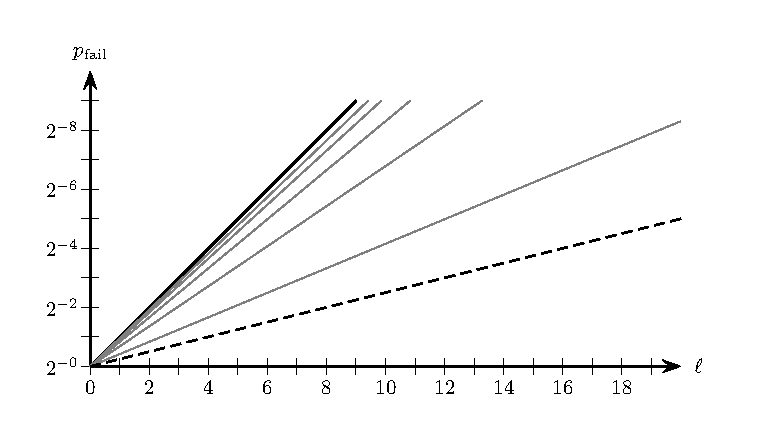
\includegraphics[scale=0.85]{figures/1106-knowledge-extraction-failure-i}
   \caption{Knowledge-extraction failure as function of iterations $\ell$. The upper black line corresponds to the verification success $\varepsilon=\frac{1}{2}$ and the lower dashed line corresponds to the lower bound obtained through the expected running-time. Grey lines between are the exact bounds for different values of $\varepsilon_\circ\in\set{2^{-2},2^{-3}, 2^{-4}, 2^{-5}, 2^{-6}}$. Clearly, the lower bound based on the expected running time is quite loose and the effect on the failure probability is marginal when $\varepsilon_\circ\ll \varepsilon$.}
   \label{fig:knowledge-extraction-failure-bounds}
\end{figure}


\paragraph{Non-standard analysis.}
Let us again start by contrasting what happens in the single cycle with the protocol execution. For that we use the same games as in the standard analysis:
\begin{align*}
 & \begin{game}{\GAME_0^{\VVV_*}}
   & \PK\gets\GEN\\
   & \overline{b}\gets \set{0,1}\\
   & (\overline{c},\overline{d})\gets\COM_\PK(\overline{b})\\
   & (b,r)\gets\VVV_*(\PK,\overline{c})\\
   & \RETURN [c\iseq r^2v^b] 
 & \end{game}
 & \begin{game}{\GAME_1^{\VVV_*}}
   & \PK\gets\GEN\\
   & \overline{b}\gets\ISQNR_{p,q}(c)\\
   & (\overline{c},\overline{d})\gets\COM_\PK(\overline{b})\\
   & (b,r)\gets\VVV_*(\PK,\overline{c})\\
   & \RETURN [c\iseq r^2v^b] \enspace.
 & \end{game}
\end{align*} 
Since $\overline{b}$ is generated randomly on the left, its value will coincide with the correct value on the left with probability $\frac{1}{2}$. Consequently, if $\varepsilon=\varepsilon(\phi,\omega)$ is the probability that $\VVV_*(\phi,\omega)$ passes the knowledge proof (verification $c=r^2v^b$), then  one iteration of the knowledge extractor will succeed with probability
\begin{align*}
\pr{\smash{\GAME_0^{\VVV_*}=1}}\geq\frac{1}{2}\cdot \pr{\smash{\GAME_1^{\VVV_*}=1}} = \frac{\varepsilon}{2}\enspace.
\end{align*}
Hence, the expected running time of a knowledge extractor is twice as slower than in standard case:
\begin{align*}
\tau=\frac{2}{\varepsilon}\enspace
\end{align*}
and the probability that the knowledge extractor fails after $\ell$ tries
\begin{align*}
\PFAIL\leq\Bigl(1-\frac{\varepsilon}{2}\Bigr)^\ell\enspace
\end{align*}
has also comparable asymptotic behaviour in the process $\ell\to\infty$. In the range $\varepsilon_\circ\leq \varepsilon\leq 2\varepsilon_\circ$, the non-standard analysis provides actually better bounds on the failure probability.

\paragraph{Solution to the paradox.}
The analysis above established that knowledge extractor works reasonably well even if the commitment scheme is not hiding. However, it is clear that malicious verifier who creates a challenge with unknown quadratic residuosity gains new knowledge during the interaction with the honest prover -- it learns the residuosity through leaking commitment. In order to clearly pinpoint where the problem occurs in the simulation, we align real protocol execution with the simulation. For that we consider a thought experiment where the knowledge extractor in the real world without using its output. As a result, we can decompose simulated and real execution into event trees with the same shape depicted in Figure~\ref{fig:event-trees}.      

\begin{figure}[!h]
   \centering
   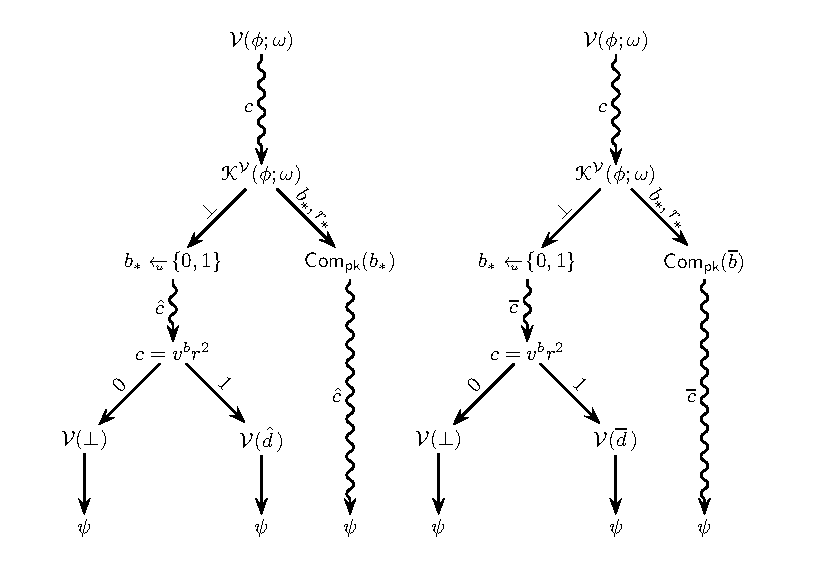
\includegraphics[scale=0.85]{figures/1106-event-tree-i}
   \caption{Event trees for the protocol simulation and for real protocol execution.}
   \label{fig:event-trees}
\end{figure}


If the knowledge extraction succeeds the simulation is perfect, since $b_*$ must coincide with $\overline{b}$. Problems occur if the simulation fails. In this case, $b_*$ is randomly chosen and corresponding commitment value is fed to the verifier $\VVV_*$, while $\VVV_*$ obtains a commitment of $\overline{b}$ in a real protocol run. If the commitment is non-hiding the difference in the commitment strings is enough to disturb the output of $\VVV_*$. In the extreme case where the commitment is perfectly hiding,  $\hat{c}$ and  $\overline{c}$ have the same distribution. Consequently, the simulation is perfect until the  simulator is forced to open $\hat{c}$. The latter does not occur, if the verifier fails to release consistent values of $r,b$, This corresponds to the left-most path on the event tree.   

Hence, we have established that the simulation might fail only for the middle path if the commitment is perfectly hiding. For brevity, let $\SFAIL$ denote the event that the knowledge error fails while verification succeeds. Then it is easy to prove that the statistical distance between the output distributions of real world execution and simulation is
\begin{align*}
\pr{\SFAIL}=\varepsilon\cdot \PFAIL = \varepsilon(1-\varepsilon)^\ell\enspace\leq \frac{1}{\ell}\cdot\left(1-\frac{1}{\ell+1}\right)^{\ell+1}\approx \frac{1}{\ell e},
\end{align*} 
which guaranteed to be negligible for reasonably chosen $\ell$.

\paragraph{Detailed analysis.}
The analysis above highlighted why the commitment must be hiding but did not quantify how much non-perfect hiding changes the bounds. Before, we go into the analysis recall a useful  bound on the distinguishing advantage. If the distribution is generated by a two-stage sampling procedure:
\begin{align*}
\ADVIND{f,g}{\AD}=\abs{\pr{\omega\gets\Omega, \psi\gets f(\omega): \AD(\psi)=1}- \pr{\omega\gets\Omega, \psi\gets g(\omega): \AD(\psi)=1 }}
\end{align*} 
then the advantage can be bounded  
\begin{align*}
\ADVIND{f,g}{\AD}\leq \sum_{\omega\in\Omega}\pr{\omega}\ADVIND{f(\omega),g(\omega)}{\AD}
\leq \max_{\omega\in\Omega} \ADVIND{f(\omega),g(\omega)}{\AD}
\end{align*} 
where a sub-advantages are defined naturally:
\begin{align*}
\ADVIND{f(\omega),g(\omega)}{\AD}=\abs{\pr{\psi\gets f(\omega): \AD(\psi)=1}- \pr{\psi\gets g(\omega): \AD(\psi)=1 }}\enspace
\end{align*}
and thus if all sub-distributions are $(\tau,\varepsilon_*)$-indistinguishable then so is the main distribution.  

Hence, it is sufficient to consider the sub-distributions where $\omega$ is fixed. Let $\AD$ be a $\tau$-time distinguisher for the verifiers output. Since the sampling procedure is still a two-stage procedure, where in the stage the knowledge-extractors output is generated, we can consider sub-distributions generated for different knowledge extractor outputs. If the output is different from $\bot$ then $b_*=\overline{c}$ and the distributions are identical. If the knowledge extractor fails, we are left with procedures
\begin{align*}
\begin{fblock}{D_1}
 & c\gets\VVV_*(\phi;\omega)\\
 & b_*\getsu \set{0,1}\\
 & \PK\gets\GEN\\
 & (\hat{c},\hat{d})\gets\COM_\PK(b_*)\\
 & r,b\gets\VVV_*(\PK,\hat{c})\\
 & \IF r^2b=c\ \THEN \RETURN \VVV_*(\hat{d}\,)\\ 
 & \ELSE \RETURN \VVV_*(\bot)
\end{fblock}
\qquad\qquad
\begin{fblock}{D_2}
 & c\gets\VVV_*(\phi;\omega)\\
 & \overline{b}\gets\ISQNR_{p,q}(c)\\
 & \PK\gets\GEN\\
 & (\overline{c},\overline{d})\gets\COM_\PK(\overline{b})\\
 & r,b\gets\VVV_*(\PK,\overline{c})\\
 & \IF r^2b=c\ \THEN \RETURN \VVV_*(\overline{d}\,)\\ 
 & \ELSE \RETURN \VVV_*(\bot)
\end{fblock}
\end{align*} 
which output we want to distinguish. This could still be viewed as a two-stage sampling procedure, where in the first stage $\beta_*\getsu\set{0,1}$ is drawn and on the second stage it is used to further (in the right game the value of $b_*$ is ignored). There are two sub-game pairs in one $b_*=\overline{b}$ and in the other they are different. Since the game pair is indistinguishable, we have to look only the second game pair. As the order of the games does not change the distinguishability, it is sufficient to estimate the distance of the following games:
\begin{align*}
\begin{fblock}{D_3}
 & c\gets\VVV_*(\phi;\omega)\\
 & \PK\gets\GEN\\
 & (\hat{c},\hat{d})\gets\COM_\PK(0)\\
 & r,b\gets\VVV_*(\PK,\hat{c})\\
 & \IF r^2b=c\ \THEN \RETURN \VVV_*(\hat{d}\,)\\ 
 & \ELSE \RETURN \VVV_*(\bot)
\end{fblock}
\qquad\qquad
\begin{fblock}{D_4}
 & c\gets\VVV_*(\phi;\omega)\\
 & \PK\gets\GEN\\
 & (\overline{c},\overline{d})\gets\COM_\PK(1)\\
 & r,b\gets\VVV_*(\PK,\overline{c})\\
 & \IF r^2b=c\ \THEN \RETURN \VVV_*(\overline{d}\,)\\ 
 & \ELSE \RETURN \VVV_*(\bot)\enspace.
\end{fblock}
\end{align*} 
Let $\AD$ be a $\tau$-time distinguisher. Then we can decompose its advantage   
\begin{align*}
\ADVIND{D_3,D_4}{\AD}\leq& \abs{\pr{\psi\gets D_3:\AD(\psi)=1\wedge r^2b\neq c}-\pr{\psi\gets D_4:\AD(\psi)=1\wedge r^2b\neq c }}\\
&+\abs{\pr{\psi\gets D_3:\AD(\psi)=1\wedge r^2b= c}-\pr{\psi\gets D_4:\AD(\psi)=1\wedge r^2b= c }}\enspace. 
\end{align*}  
If the running time $t_{v}$ of $\VVV_*$ is small enough so that the total running time of $D_3$ and $D_4$ without the first if branch is below $t$ then 
\begin{align*}
\abs{\pr{\psi\gets D_3:\AD(\psi)=1\wedge r^2b\neq c}-\pr{\psi\gets D_3:\AD(\psi)=1\wedge r^2b\neq c }}\leq \varepsilon_\circ\enspace,
\end{align*}  
or otherwise we can use the adversary 
\begin{align*}
\begin{aligned}
\begin{fblock}{\AD(\PK)}
 & c\gets\VVV_*(\phi;\omega)\\
 &\RETURN (0,1)\\
\end{fblock}\\
 \\
\end{aligned}
\qquad\qquad
\begin{fblock}{\AD(c)}
 & r,b\gets\VVV_*(\PK,\overline{c})\\
 & \IF r^2b=c\ \THEN \RETURN \bot\\ 
 & \ELSE \RETURN \ADB(\VVV_*(\bot))
\end{fblock}
\end{align*}
as the $t$-time distinguisher against hiding games. For the second term we use just a trivial upper bound. As a result, we get
\begin{align*}
\ADVIND{D_3,D_4}{\AD}\leq&\max\set{\pr{\psi\gets D_3:r^2b=c},\pr{\psi\gets D_4: r^2b=c}}+\varepsilon_\circ\enspace. 
\end{align*}  
However, the cannot bound the probabilities under the maximum operator, the malicious verifier can have arbitrary success in releasing $r,b$. Hence, we cannot eliminate knowledge extraction from the distribution generation in order to get reasonable bound on the distinguishing advantage. 

As a result we have to analyse the computational distance of following distributions
\begin{align*}
\begin{fblock}{D_1}
 & c\gets\VVV_*(\phi;\omega)\\
 & \overline{b}\gets\ISQNR_{p,q}(c)\\
 & (b_*,r_*)\gets\KEXTR^{\VVV_*}(\phi,\ell;\omega)\\
 & \IF (b_*,r_*)=\bot\ \THEN  b_*\getsu \set{0,1}\\
 & \PK\gets\GEN\\
 & (\hat{c},\hat{d})\gets\COM_\PK(b_*)\\
 & r,b\gets\VVV_*(\PK,\hat{c})\\
 & \IF r^2b=c\ \THEN \RETURN \VVV_*(\hat{d}\,)\\ 
 & \ELSE \RETURN \VVV_*(\bot)
\end{fblock}
\qquad\qquad
\begin{fblock}{D_2}
 & c\gets\VVV_*(\phi;\omega)\\
 & \overline{b}\gets\ISQNR_{p,q}(c)\\
 & (b_*,r_*)\gets\KEXTR^{\VVV_*}(\phi,\ell;\omega)\\
 & \IF (b_*,r_*)=\bot\ \THEN  b_*\getsu \set{0,1}\\
 & \PK\gets\GEN\\
 & (\overline{c},\overline{d})\gets\COM_\PK(\overline{b})\\
 & r,b\gets\VVV_*(\PK,\overline{c})\\
 & \IF r^2b=c\ \THEN \RETURN \VVV_*(\overline{d}\,)\\ 
 & \ELSE \RETURN \VVV_*(\bot)\enspace
\end{fblock}
\end{align*} 
where the distribution corresponding to the ideal execution ignores the value $\overline{b}$ and the distribution corresponding to the real execution ignores the value $b_*$. As before view can view the sampling procedure as a two-stage procedure where in the first phase $b_*$ is sampled. Hence, we can consider two sub-distributions. One with $b_*=\overline{b}$ and the other with $b_*\neq\overline{b}$. As distributions are identical  in the first case, we must analyse only the distance between 
\begin{align*}
\begin{fblock}{D_3}
 & c\gets\VVV_*(\phi;\omega)\\
 & \overline{b}\gets\ISQNR_{p,q}(c)\\
 & (b_*,r_*)\gets\KEXTR^{\VVV_*}(\phi,\ell;\omega)\\
 & \IF (b_*,r_*)=\bot\ \THEN  b_*\getsu \neg \overline{b}\\
 & \PK\gets\GEN\\
 & (\hat{c},\hat{d})\gets\COM_\PK(b_*)\\
 & r,b\gets\VVV_*(\PK,\hat{c})\\
 & \IF r^2b=c\ \THEN \RETURN \VVV_*(\hat{d}\,)\\ 
 & \ELSE \RETURN \VVV_*(\bot)
\end{fblock}
\qquad\qquad
\begin{fblock}{D_4}
 & c\gets\VVV_*(\phi;\omega)\\
 & \overline{b}\gets\ISQNR_{p,q}(c)\\
 & (b_*,r_*)\gets\KEXTR^{\VVV_*}(\phi,\ell;\omega)\\
 & \IF (b_*,r_*)=\bot\ \THEN  b_*\getsu \neg \overline{b}\\
 & \PK\gets\GEN\\
 & (\overline{c},\overline{d})\gets\COM_\PK(\overline{b})\\
 & r,b\gets\VVV_*(\PK,\overline{c})\\
 & \IF r^2b=c\ \THEN \RETURN \VVV_*(\overline{d}\,)\\ 
 & \ELSE \RETURN \VVV_*(\bot)\enspace
\end{fblock}
\end{align*} 
Note that for fixed $\phi,\omega$ pair, the knowledge extractor fails with the same but probability $\PFAIL=\PFAIL(\VVV_*)$. Hence, we can simplify the distributions: 
\begin{align*}
\begin{fblock}{D_5}
 & c\gets\VVV_*(\phi;\omega)\\
 & \overline{b}\gets\ISQNR_{p,q}(c)\\
 & s\getsu [0,1]\\
 & \IF s\leq \PFAIL(\VVV_*)\ \THEN  b_*\getsu \neg \overline{b}\\
 & \ELSE b_*\gets \overline{b}\\
 & \PK\gets\GEN\\
 & (\hat{c},\hat{d})\gets\COM_\PK(b_*)\\
 & r,b\gets\VVV_*(\PK,\hat{c})\\
 & \IF r^2b=c\ \THEN \RETURN \VVV_*(\hat{d}\,)\\ 
 & \ELSE \RETURN \VVV_*(\bot)
\end{fblock}
\qquad\qquad
\begin{fblock}{D_6}
 & c\gets\VVV_*(\phi;\omega)\\
 & \overline{b}\gets\ISQNR_{p,q}(c)\\
 & s\getsu [0,1]\\
 & \IF s\leq \PFAIL(\VVV_*)\ \THEN  b_*\getsu \neg \overline{b}\\
 & \ELSE b_*\gets \overline{b}\\
 & \PK\gets\GEN\\
 & (\overline{c},\overline{d})\gets\COM_\PK(\overline{b})\\
 & r,b\gets\VVV_*(\PK,\overline{c})\\
 & \IF r^2b=c\ \THEN \RETURN \VVV_*(\overline{d}\,)\\ 
 & \ELSE \RETURN \VVV_*(\bot)\enspace.
\end{fblock}
\end{align*} 
Let $\AD$ be a $\tau$-time distinguisher. Then we can decompose its advantage   
\begin{align*}
\ADVIND{D_3,D_4}{\AD}\leq& \abs{\pr{\psi\gets D_3:\AD(\psi)=1\wedge r^2b\neq c}-\pr{\psi\gets D_4:\AD(\psi)=1\wedge r^2b\neq c }}\\
&+\abs{\pr{\psi\gets D_3:\AD(\psi)=1\wedge r^2b= c}-\pr{\psi\gets D_4:\AD(\psi)=1\wedge r^2b= c }}\enspace. 
\end{align*}  
Let us first analyse the second term $\Delta_2$.  Clearly, if $s > \PFAIL(\VVV_*)$ then the distributions provide identical outputs and thus the advantage of $\AD$ can be expressed by the following games:
\begin{align*}
\begin{fblock}{\GAME_0^\AD}
 & c\gets\VVV_*(\phi;\omega)\\
 & \overline{b}\gets\ISQNR_{p,q}(c)\\
 & s\getsu [0,1]\\
 & \IF s> \PFAIL(\VVV_*)\ \THEN \RETURN 0\\
 & b_*\getsu \neg \overline{b}\\
 & \PK\gets\GEN\\
 & (\hat{c},\hat{d})\gets\COM_\PK(b_*)\\
 & r,b\gets\VVV_*(\PK,\hat{c})\\
 & \IF r^2b=c\ \THEN \RETURN \AD(\VVV_*(\hat{d}\,))\\ 
 & \ELSE \RETURN 0
\end{fblock}
\qquad\qquad
\begin{fblock}{\GAME_1^\AD}
 & c\gets\VVV_*(\phi;\omega)\\
 & \overline{b}\gets\ISQNR_{p,q}(c)\\
 & s\getsu [0,1]\\
 & \IF s> \PFAIL(\VVV_*)\ \THEN \RETURN 0\\
 & b_*\getsu \neg \overline{b}\\
 & \PK\gets\GEN\\
 & (\overline{c},\overline{d})\gets\COM_\PK(\overline{b})\\
 & r,b\gets\VVV_*(\PK,\overline{c})\\
 & \IF r^2b=c\ \THEN \RETURN \AD(\VVV_*(\overline{d}\,))\\ 
 & \ELSE \RETURN 0\enspace.
\end{fblock}
\end{align*}
Now, it is evident that we have to consider only the probability differences in the branches $s>\PFAIL$ and thus 
\begin{align*}
\Delta_2=\PFAIL\cdot\abs{\pr{\GAME_2^\AD=1}-\pr{\GAME_3^\AD=1}}
\end{align*}
where 
\begin{align*}
\begin{fblock}{\GAME_2^\AD}
 & c\gets\VVV_*(\phi;\omega)\\
 & \PK\gets\GEN\\
 & (\hat{c},\hat{d})\gets\COM_\PK(0)\\
 & r,b\gets\VVV_*(\PK,\hat{c})\\
 & \IF r^2b=c\ \THEN \RETURN \AD(\VVV_*(\hat{d}\,))\\ 
 & \ELSE \RETURN 0
\end{fblock}
\qquad\qquad
\begin{fblock}{\GAME_3^\AD}
 & c\gets\VVV_*(\phi;\omega)\\
 & \PK\gets\GEN\\
 & (\hat{c},\hat{d})\gets\COM_\PK(1)\\
 & r,b\gets\VVV_*(\PK,\overline{c})\\
 & \IF r^2b=c\ \THEN \RETURN \AD(\VVV_*(\hat{d}\,))\\ 
 & \ELSE \RETURN 0\enspace.
\end{fblock}
\end{align*}
From these games it is evident that 
\begin{align*}
\abs{\pr{\GAME_2^\AD=1}-\pr{\GAME_3^\AD=1}}\leq \max\set{\pr{r,b\gets D_7: r^2v^b=c}, \pr{r,b\gets D_8: r^2v^b=c}}
\end{align*}
where procedure $D_7$ and $D_8$ correspond to the first fragments of the game:
\begin{align*}
\begin{fblock}{D_7}
 & c\gets\VVV_*(\phi;\omega)\\
 & \PK\gets\GEN\\
 & (\hat{c},\hat{d})\gets\COM_\PK(0)\\
 & r,b\gets\VVV_*(\PK,\hat{c})\\
 & \RETURN (r,b)
\end{fblock}
\qquad\qquad
\begin{fblock}{D_8}
 & c\gets\VVV_*(\phi;\omega)\\
 & \PK\gets\GEN\\
 & (\hat{c},\hat{d})\gets\COM_\PK(1)\\
 & r,b\gets\VVV_*(\PK,\hat{c})\\
 & \RETURN (r,b)\enspace.
\end{fblock}
\end{align*}
If the running time $t_v$ of $\VVV_*$ together with the running time $\tau$ of $\AD$ is below $t$, then the advantages corresponding to these games can differ only by $\varepsilon_\circ$. As one of these runs corresponds to the same fragment is  the real world execution and has thus probability $\varepsilon$, we have established that
\begin{align*}
\abs{\pr{\GAME_2^\AD=1}-\pr{\GAME_3^\AD=1}}\leq \varepsilon +\varepsilon_\circ\enspace.
\end{align*}
This implies
\begin{align*}
\ADVIND{D_3,D_4}{\AD}\leq& \abs{\pr{\psi\gets D_3:\AD(\psi)=1\wedge r^2b\neq c}-\pr{\psi\gets D_4:\AD(\psi)=1\wedge r^2b\neq c }}+ \PFAIL(\VVV_*)\cdot(\varepsilon+\varepsilon_\circ)\enspace. 
\end{align*}
To estimate the remaining term, we can consider the following games   
\begin{align*}
\begin{fblock}{\GAME_5^\AD}
 & c\gets\VVV_*(\phi;\omega)\\
 & \overline{b}\gets\ISQNR_{p,q}(c)\\
 & s\getsu [0,1]\\
 & \IF s> \PFAIL(\VVV_*)\ \THEN \RETURN 0\\
 & b_*\getsu \neg \overline{b}\\
 & \PK\gets\GEN\\
 & (\hat{c},\hat{d})\gets\COM_\PK(b_*)\\
 & r,b\gets\VVV_*(\PK,\hat{c})\\
 & \IF r^2b=c\ \THEN \RETURN 0\\ 
 & \ELSE \RETURN \AD(\VVV_*(\bot))
\end{fblock}
\qquad\qquad
\begin{fblock}{\GAME_6^\AD}
 & c\gets\VVV_*(\phi;\omega)\\
 & \overline{b}\gets\ISQNR_{p,q}(c)\\
 & s\getsu [0,1]\\
 & \IF s> \PFAIL(\VVV_*)\ \THEN \RETURN 0\\
 & b_*\getsu \neg \overline{b}\\
 & \PK\gets\GEN\\
 & (\overline{c},\overline{d})\gets\COM_\PK(\overline{b})\\
 & r,b\gets\VVV_*(\PK,\overline{c})\\
 & \IF r^2b=c\ \THEN \RETURN 0\\ 
 & \ELSE \RETURN \AD(\VVV_*(\bot))\enspace.
\end{fblock}
\end{align*}
Clearly the difference can only grow if we omit the first check and consider games
\begin{align*}
\begin{fblock}{\GAME_7^\AD}
 & c\gets\VVV_*(\phi;\omega)\\
 & \PK\gets\GEN\\
 & (\hat{c},\hat{d})\gets\COM_\PK(0)\\
 & r,b\gets\VVV_*(\PK,\hat{c})\\
 & \IF r^2b=c\ \THEN \RETURN 0\\ 
 & \ELSE \RETURN \AD(\VVV_*(\bot))
\end{fblock}
\qquad\qquad
\begin{fblock}{\GAME_8^\AD}
 & c\gets\VVV_*(\phi;\omega)\\
 & \PK\gets\GEN\\
 & (\hat{c},\hat{d})\gets\COM_\PK(0)\\
 & r,b\gets\VVV_*(\PK,\hat{c})\\
 & \IF r^2b=c\ \THEN \RETURN 0\\ 
 & \ELSE \RETURN \AD(\VVV_*(\bot))\enspace.
\end{fblock}
\end{align*}
As the decommitment value is never released, we can reduce these games to hiding game. Thus 
if the sum of running times $t_v+\tau\leq t$, then
\begin{align*}
\abs{\pr{\GAME_7^\AD=1}-\pr{\GAME_8^\AD=1}}\leq \varepsilon_\circ\enspace,
\end{align*}
which leads to the following final estimate:
\begin{align*}
\ADVIND{D_3,D_4}{\AD}\leq \varepsilon_\circ + \PFAIL(\VVV_*)\cdot(\varepsilon+\varepsilon_\circ)\enspace. 
\end{align*}

\paragraph{Final remarks.}
Let us now compare the results for perfectly hiding and computationally hiding commitments. Let $\psi$ denote the outdot distribution for the real and $\psi_\circ$ the output distribution for the simulation. Then we can express the bounds on the distinguishing advantage as follows:
\begin{align*}
\SD(\psi,\psi_\circ)&\leq\max_{\varepsilon\in[0,1]} \varepsilon(1-\varepsilon)^\ell\\
\CD^\tau(\psi,\psi_\circ)&\leq \varepsilon_\circ +\max_{\varepsilon\in[0,1]}(\varepsilon+\varepsilon_\circ)(1+\varepsilon_\circ-\varepsilon)^\ell\enspace.
\end{align*}  
The form of the inequalities indicates that the value $\varepsilon_\circ$ influences the bound in two ways. First it offsets the final bound by the $\varepsilon_\circ$. Second, it offsets the simulation error term. This effect is bounded. One can clearly see that it can offset the second term only by $\varepsilon_\circ$ at most. 

Another thing that is worth mentioning is that our analysis excluded the complexity of the knowledge extractor. Hence, by increasing $\ell$ we can suppress the second term regardless of the bound $t$. Of course, this increases the overhead of simulator and thus is unwanted but at least we do not have to choose the commitment scheme parameters on planned overhead.


\end{solution}
\end{document}

